 %\pdfoutput=1
\documentclass[conference]{IEEEtran}
\IEEEoverridecommandlockouts
% The preceding line is only needed to identify funding in the first footnote. If that is unneeded, please comment it out.
\usepackage[T1]{fontenc}
\usepackage{cite}
\usepackage{mathtools}
\usepackage{stackengine}
\def\delequal{\mathrel{\ensurestackMath{\stackon[1pt]{=}{\scriptstyle\Delta}}}}
\usepackage{amsmath,amssymb,amsfonts}
\usepackage{amsmath,epsfig,cite,amsfonts,amssymb,psfrag,subfig}
\usepackage{graphicx}
\usepackage{textcomp}
\usepackage{xcolor}
\usepackage{algorithm}
\usepackage[noend]{algpseudocode}
\usepackage{amsthm}
\def\BibTeX{{\rm B\kern-.05em{\sc i\kern-.025em b}\kern-.08em
    T\kern-.1667em\lower.7ex\hbox{E}\kern-.125emX}}
\allowdisplaybreaks
\newtheorem{remark}{Remark}
\newtheorem{theorem}{Theorem}
\newtheorem{lemma}{Lemma}
\newtheorem{proposition}{Proposition}
\newtheorem{corollary}{Corollary}
\newcommand{\diag}{\mathop{\mathrm{diag}}}
\DeclareMathOperator{\E}{\mathbb{E}}
\usepackage[margin=0.7in]{geometry}
\setlength{\columnsep}{11mm}
\begin{document}

\title{Network Slicing and Resource Allocation in an Open RAN System \vspace{-.1cm}
}
%
%\author{\IEEEauthorblockN{1\textsuperscript{st} Mojdeh Karbalaee Motalleb}
%\IEEEauthorblockA{\textit{Electrical and Computer Engineering} \\
%\textit{Tehran University}\\
%Tehran, Iran \\
%mojdeh.karbalaee@ut.ac.ir}
%\and
%\IEEEauthorblockN{2\textsuperscript{nd} Vahid Shah-Mansouri}
%\IEEEauthorblockA{\textit{Electrical and Computer Engineering} \\
%\textit{Tehran University}\\
%Tehran, Iran \\
%vmansouri@ut.ac.ir}
%\and
%\IEEEauthorblockN{3\textsuperscript{rd} Salar Nouri Naghadeh}
%\IEEEauthorblockA{\textit{Electrical and Computer Engineering} \\
%\textit{Tehran University}\\
%Tehran, Iran \\
%salar.nouri@ut.ac.ir}
%}
%%%%%  \author{
%%%%%    \IEEEauthorblockN{Mojdeh Karbalaee Motalleb}
%%%%%    \IEEEauthorblockA{School of ECE, College of Engineering, University of Tehran, Iran \\
%%%%%    Email: \{mojdeh.karbalaee\}@ut.ac.ir,
%%%%%    \vspace{-.2cm}
%%%%%  }
%%%%%  }

\maketitle

\begin{abstract}

\end{abstract}
\section{Introduction} 

\begin{figure*}
  \centering 
    \includegraphics[scale = 0.5]{finalDraw.pdf}
    %\includegraphics[max height=30cm,max width=9.5cm]{Drawing15.eps}
    %\includegraphics[width=\textwidth]{finalDraw.pdf}
  \caption{Network sliced ORAN system}
  \label{fig:c11}
\end{figure*}



\section{System Model and Problem Formulation}
\subsection{System Model}
%This paper deals with the challenges of heterogeneous vehicular and cellular networks.
Assume we have two preallocated slices serving two services, eMBB, and URLLC services; 
eMBB Service consists of $U_{1}$ single-antenna user equipments (UEs) and URLLC service consists of $U_2$ UEs.
Assume our system consists of $K$, preallocated physical resource blocks (PRBs). Moreover, the system considers to have $M_s^{d}$ VNFs for the processing of O-DU, $M_s^{c}$ VNFs for the processing of O-CU-UP of eMBB and URLLC ($ s \in \{1, 2\}$). 
Virtual network functions (VNFs) are functional blocks of the system. Each VNF instance runs on a virtual machine (VM) using resources from the data centers. 
Moreover, we assume there is a cell with one multi-antenna O-RU that serves UEs.
\subsection{The Achievable Rate}
The eMBB services typically use more than a one-time slot. But URLLC services use part of a time slot (mini-slot) since it has short packet transmission. In addition, the URLLC must be punctured as soon as it has requested service as it requires very low latency.


%The SNR of $i^{th}$ UE requesting served at slice $ss \in \{1, 2\}$ is obtained from
%\begin{equation}\label{eq2}
%\rho_{u(s,i)} =  \frac{\sum_{k=1}^{K_{s}}e_{u(s,i)}^k p_{u(s,i)}^{k}|{\bold{h}_{R,u(s,i)}^{H \: k}}|^2}{BN_0},
%\end{equation} 
%where $p_{u(s,i)}^{k}$ represents the transmission power allocated by O-RUs to $i^{th}$ UE served at slice $s$ on PRB $k$.
%${\bold{h}_{R,u(s,i)}^{k}} \in \mathbb{C}^{R}$ is the vector of channel gain of a wireless link from 
%O-RUs to the $i^{th}$ UE in $s^{th}$ slice. 
%Moreover, $e_{u(s,i)}^k \in \{0,1\}$ is a binary variable that illustrates whether PRB $k$ is assigned to the $i^{th}$ UE allocated to $s^{th}$ slice or not. 
%Also, $BN_0$ denotes the power of Gaussian additive noise.
%Moreover, we assume that each PRB is assigned to no more than one UEs. So we have
%\begin{equation}
%\sum_{s=1}^S \sum_{u=1}^{U_s} e_{u(s,i)}^k = 1
%\end{equation} 
The achievable data rate for the $i^{th}$ UE request eMBB slice can be written as $\mathcal{R}_{i}^{e}(t)$.
\begin{equation}\label{eq1}
\mathcal{R}_{i}^e(t) = \sum_{k = 1}^K e^k_i(t) B (1-\frac{n^k_i(t)}{S}) \log_2({1+\frac{p^k_i(t)h^k_i(t)}{B \times N_0}}),
\end{equation}
where $B$ is the bandwidth of RBs. Also, $B\times N_0$ denotes the power of Gaussian additive noise. 
Moreover, $e^k_i(t)\in \{0,1\}$ is a binary variable that illustrates whether PRB $k$ is assigned to the $i^{th}$ eMBB UE or not. 
$p^k_i(t)$ represents the transmission power allocated by O-RU to $i^{th}$ UE of eMBB using PRB $k$.
$h^k_i(t)$ is the channel gain of a wireless link from 
O-RU to the $i^{th}$ eMBB UE using $k^{th}$ PRB. In addition, $S$ is the total number of mini-slots of a PRB. 
Furthermore, $n^k_i(t)$ is the number of URLLC punctured slots. 

Since the blocklength in URLLC is finite, the achievable data rate for the $j^{th}$ UE request in the URLLC service, is not achieved from Shannon Capacity formula. So, for the short packet transmission the achievable data rate is approximated as follow
\begin{equation}\label{eq11}
\mathcal{R}_{j}^u(t) = \sum_{i = 1}^{U_1}\sum_{k=1}^K \frac{n^k_i(t)e^k_i(t)}{S \times U_2} B \log_2({1+\frac{p^k_j(t)h^k_j(t)}{B \times N_0}})- \zeta_{j}^k(t)), 
\end{equation}

where $\zeta_{j}^k(t) = \log_2({e})Q^{-1}(\epsilon) \sqrt{\frac{C_{j}^k(t)}{N_{j}^k(t)}})$
where $\epsilon$ is the transmission error probability, $Q^{-1}$ is the inverse of Q function (i.e., Gaussian),
$C_{j}^k(t) = 1 - \frac{1}{(1+\rho_{j}^k(t))^2}$ depicts the channel dispersion of UE $j$ of URLLC, puncturing mini-slots of PRB $k$ and
$N_{j}^k(t)$ represents the blocklength of it. Moreover, $\rho_{j}^k(t)=\frac{p^k_j(t)h^k_j(t)}{B \times N_0}$ is the SNR of UE $j$ in URLLC service. 

The channel gain is assumed to be known with errors, the imperfection of channel estimation is
modeled as follows
\begin{equation}
h^k_j(t) = \hat{h}^k_j(t) + \Delta h^k_j(t)
\end{equation}
Where, $\Delta h^k_j(t)$ denotes the estimation error with a Guassian distribution of
 \begin{equation}
\Delta h^k_j(t)\backsim \mathcal{N}(0,\boldsymbol{\phi^k}^2),
\end{equation}
\subsection{Mean Delay}
In this part, the mean processing delay for each service is obtained.
Suppose the mean processing delay is depicted as $T_{\text{\text{proc}}}$,
\begin{equation}
T^{\text{proc}} =  T^{RU} + T^{DU} + T^{CU},
\end{equation}
Assume the packet arrival of URLLC UEs follows a Poisson process with arrival rate $\lambda_{j}$ for the $j^{th}$ UE.
Therefore, the mean arrival data rate of the O-CU-UP layer is $\alpha^C = \sum_{j=1}^{U_2}\lambda_{j}$.
Assume the mean arrival data rate for URLLC slice ($\alpha$) is approximately equal to the mean arrival data rate of the  the O-DU ($\alpha^D$). so $\alpha = \alpha^C \approx \alpha^D$,
Because the amount of data traffic transferred along the route (regardless of frame changes) is constant.
Since, by using Burke’s theorem, the mean arrival data rate of the second layer, which are processed in the first layer, is still poisson with rate $\alpha$.
It is assumed that there are load balancers in each layer for each service to divide the incoming traffic to VNFs equally. %\cite{frdl,luong2018novel,luong2018novel1}.
Suppose the baseband processing of each VNF is depicted as M/M/1 processing queue.
Each packet is processed by one of the VNFs of a slice. So, the mean delay for the URLLC slice in the O-DU,and the O-CU is modeled as M/M/1 queue, is formulated as follows, respectively \cite{SystemCostMinimization,luong2018joint,luong2018novel},
\begin{equation}
\begin{split}
T^{DU} &= \frac{1}{\mu^d - \alpha/{M^{d}}},\\
T^{CU} &= \frac{1}{\mu^c - \alpha/{M^{c}}},\\
\end{split}
\end{equation}
where $M^{d}$,and $M^{c}$ are the variables that depict the number of VNFs in O-DU,and O-CU-UP, respectively. 
Moreover, $1/\mu^d$, and $1/\mu^c$ are the mean service time of the O-DU, and O-CU layers, respectively.
Besides, $\alpha$ is the  arrival rate which is divided
by load balancer before arriving to the VNFs. The arrival rate of each VNF in each layer for URLLC slice  is $\alpha/{M^{l}}$ $ l \in \{d,c\}$.

$T_{j}^{RU}$ is the mean transmission delay of the $j^{th}$ UE of the URLLC service on the wireless link.
 The arrival data rate of wireless link for each UE $j$ of URLLC service is $\lambda_j$
As a result, we have $\sum_{j = 1}^{U_2} \lambda_{j} = \alpha$.
Moreover, The service time of transmission queue for UE $j$ requesting URLLC service has
an exponential distribution with mean $1/R_{j}^u$ and can be modeled as a M/M/1 queue \cite{SystemCostMinimization,luong2018joint,luong2018novel}.
 
Therefore, the mean delay of the transmission layer for UE $j$ in URLLC slice is
\begin{equation}
 T_{j}^{RU} = \frac{1}{R_{j}^u - \lambda_{j}}.
\end{equation}


\subsection{Reliability of URLLC}
As we know, UEs request URLLC services, require services with low latency.
For the M/M/1 system, the probability of the delay for URLLC service in the O-RU is as follow, 
\begin{equation}
P_r\{T_{j}^{RU} \geq T_{RU}^{max}\} = e^{-(R_{tot}^u - \alpha)T_{RU}^{max}}
\end{equation} 
where, $R_{tot}^u = \sum_{j =1}^{U_2}R_{j}^u$
Also, we do not consider the reliability for O-CU and O-DU.

\subsection{Problem Statement}
%In this system, the goal is to minimize the cost of the system.
%The total power cost of O-RUs for transmitting data to UE is depicted as follow
%\begin{equation}
%P_{tot} = \sum_{r=1}^{R}P_r
%\end{equation}
The optimization problem is formulated as follow

\begin{subequations} \label{mainP}
\begin{alignat}{4}
\max\limits_{ \boldsymbol{E}, \boldsymbol{N},\boldsymbol{M} } &  \sum_i R_{i}^e(t) - \eta \sum_j T^{\text{proc}, u}(t)       \ \\
\text{subject to} \quad  & \mathcal{R}_{i}^e(t) \geq  \mathcal{R}_{min}^e \quad \forall i \in U_1, \label{p1} \\
& Pr\{{R}_{i}^e(t) \leq {R}_{min}^e\}  \leq \epsilon \label{p2}\\
&T^{\text{proc}, u}_j(t)  \leq T_{min}^u  \quad \forall j \in U_2 \label{p3} \\
&Pr\{T^{\text{proc}, u}_j(t) \geq T_{min}^u\} \leq \epsilon  \quad \forall j \in U_2 \label{p4} 
\end{alignat}
\label{constraints}
\end{subequations}
where, \eqref{p2}, supports the reliability of eMBB while puncturing the URLLC. 

\bibliographystyle{IEEEtran}
\bibliography{ref}
\end{document} 